%% ============================================================
%%  Real-Time Crime Analytics & Intelligent Alert System
%%  Technical Report — CS4109 Big Data Analytics
%%  FAST-NUCES Islamabad, Spring 2026
%% ============================================================
\documentclass[12pt,a4paper]{article}

%% ── Packages ──────────────────────────────────────────────
\usepackage[T1]{fontenc}
\usepackage[utf8]{inputenc}
\usepackage{lmodern}
\usepackage[margin=2.2cm,top=2.5cm,bottom=2.5cm]{geometry}
\usepackage{graphicx}
\usepackage{float}
\usepackage{caption}
\usepackage{subcaption}
\usepackage{booktabs}
\usepackage{longtable}
\usepackage{array}
\usepackage{multirow}
\usepackage{tabularx}
\usepackage{xcolor}
\usepackage{hyperref}
\usepackage{fancyhdr}
\usepackage{titlesec}
\usepackage{enumitem}
\usepackage{listings}
\usepackage{tcolorbox}
\usepackage{mdframed}
\usepackage{tikz}
\usepackage{amsmath}
\usepackage{setspace}
\usepackage{parskip}
\usepackage{microtype}
\usepackage{fontawesome5}

\usetikzlibrary{shapes.geometric, arrows.meta, positioning, fit, backgrounds}

%% ── Colours ───────────────────────────────────────────────
\definecolor{nuBlue}{RGB}{0,56,147}
\definecolor{nuGold}{RGB}{200,160,0}
\definecolor{codeGray}{RGB}{245,245,245}
\definecolor{alertRed}{RGB}{192,0,0}
\definecolor{darkGray}{RGB}{60,60,60}
\definecolor{lightBlue}{RGB}{230,240,255}
\definecolor{arrowBlue}{RGB}{30,100,200}

%% ── Hyperref ──────────────────────────────────────────────
\hypersetup{
  colorlinks=true,
  linkcolor=nuBlue,
  urlcolor=nuBlue,
  citecolor=nuBlue,
  pdftitle={Real-Time Crime Analytics \& Intelligent Alert System},
  pdfauthor={M Mobin, M Nouman Hafeez},
}

%% ── Header / Footer ──────────────────────────────────────
\pagestyle{fancy}
\fancyhf{}
\fancyhead[L]{\small\color{nuBlue}\textbf{Real-Time Crime Analytics \& Intelligent Alert System}}
\fancyhead[R]{\small\color{darkGray}CS4109 — Big Data Analytics}
\fancyfoot[C]{\small\thepage}
\fancyfoot[R]{\small\color{darkGray}FAST-NUCES Islamabad}
\renewcommand{\headrulewidth}{0.5pt}
\renewcommand{\footrulewidth}{0.3pt}

%% ── Section Formatting ────────────────────────────────────
\titleformat{\section}{\large\bfseries\color{nuBlue}}{}{0em}{}[\titlerule]
\titleformat{\subsection}{\normalsize\bfseries\color{darkGray}}{}{0em}{}
\titleformat{\subsubsection}{\normalsize\itshape\color{darkGray}}{}{0em}{}

%% ── Code Listings ─────────────────────────────────────────
\lstset{
  backgroundcolor=\color{codeGray},
  basicstyle=\ttfamily\small,
  breaklines=true,
  frame=single,
  framerule=0.4pt,
  rulecolor=\color{nuBlue!40},
  keywordstyle=\color{nuBlue}\bfseries,
  commentstyle=\color{green!50!black},
  stringstyle=\color{alertRed},
  numbers=left,
  numberstyle=\tiny\color{gray},
  numbersep=5pt,
  tabsize=2,
  captionpos=b,
}

%% ── Custom box ────────────────────────────────────────────
\tcbuselibrary{skins,breakable}
\newtcolorbox{infobox}[1][]{
  colback=lightBlue, colframe=nuBlue, fonttitle=\bfseries,
  title=#1, sharp corners, boxrule=0.6pt,
}

\graphicspath{{figs/}}

%% ════════════════════════════════════════════════════════════
\begin{document}
\pagenumbering{gobble}

%% ── COVER PAGE ───────────────────────────────────────────
\begin{titlepage}
\begin{tikzpicture}[remember picture, overlay]
  % Top bar
  \fill[nuBlue] (current page.north west) rectangle
    ([yshift=-3.2cm]current page.north east);
  % Bottom bar
  \fill[nuGold] (current page.south west) rectangle
    ([yshift=1.2cm]current page.south east);
  % Thin accent strip
  \fill[nuGold!80] ([yshift=-3.2cm]current page.north west)
    rectangle ([yshift=-3.5cm]current page.north east);
\end{tikzpicture}

\vspace*{1.4cm}

\begin{center}
  {\color{white}\Large\bfseries FAST -- National University of Computer}\\[3pt]
  {\color{white}\Large\bfseries and Emerging Sciences, Islamabad}\\[8pt]
  {\color{white}\normalsize Department of Computer Science}
\end{center}

\vspace{1.4cm}

\begin{center}
  \includegraphics[width=0.22\textwidth]{shutterstock_165692999.jpg}
  % (placeholder for NU logo — replace with actual logo if available)
\end{center}

\vspace{0.6cm}

\begin{center}
  {\color{nuBlue}\rule{0.82\linewidth}{1.5pt}}\\[10pt]
  {\Huge\bfseries\color{nuBlue} Real-Time Crime Analytics}\\[6pt]
  {\LARGE\color{darkGray}\&\ Intelligent Alert System}\\[10pt]
  {\color{nuBlue}\rule{0.82\linewidth}{1.5pt}}
\end{center}

\vspace{0.5cm}

\begin{center}
  \begin{tcolorbox}[colback=nuBlue!6,colframe=nuBlue,width=0.78\linewidth,
      sharp corners, boxrule=0.6pt]
    \centering
    {\large\bfseries Course:} CS4109 — Fundamentals of Big Data Analytics\\[4pt]
    {\large\bfseries Section:} CS-A \quad|\quad
    {\large\bfseries Session:} Spring 2026
  \end{tcolorbox}
\end{center}

\vspace{0.5cm}

\begin{center}
  \begin{tabular}{lll}
    \toprule
    \textbf{Member} & \textbf{Name} & \textbf{Roll Number}\\
    \midrule
    1 & Muhammad Mobin       & 21I-0794 \\
    2 & Muhammad Nouman Hafeez & 21I-0416 \\
    \bottomrule
  \end{tabular}
\end{center}

\vspace{0.6cm}

\begin{center}
  \begin{tabular}{ll}
    \textbf{Instructor:}  & Ms.\ Kainat Iqbal \& Dr.\ Asif Muhammad \\
    \textbf{Submission:}  & 11 May 2026, 11:59 PM \\
  \end{tabular}
\end{center}

\vfill
\begin{center}
  {\color{nuGold!60!black}\small
  ``Building something that matters — real-time public-safety intelligence for the modern city.''}
\end{center}
\vspace{0.3cm}

\end{titlepage}

\pagenumbering{roman}
\setcounter{page}{1}

%% ── TABLE OF CONTENTS ────────────────────────────────────
\tableofcontents
\newpage

\pagenumbering{arabic}
\setcounter{page}{1}

% ═══════════════════════════════════════════════════════════════
\section{Introduction}
% ═══════════════════════════════════════════════════════════════

Urban crime analysis is a critical challenge for public-safety agencies. Traditional batch reporting systems are insufficient for time-sensitive decision-making. Modern cities require intelligent, real-time analytics pipelines capable of detecting anomalies, identifying hotspots, and dispatching alerts as incidents unfold.

This project implements a \textbf{Real-Time Crime Analytics and Intelligent Alert System} powered by the City of Chicago's publicly available public-safety datasets. Using a \textbf{Lambda Architecture}, the system simultaneously supports:

\begin{itemize}[leftmargin=1.6em]
  \item \textbf{Batch processing} — historical trend analysis, machine learning, and cross-dataset joins using Apache Spark.
  \item \textbf{Stream processing} — real-time event ingestion, windowed anomaly detection, and alert generation using Apache Kafka and Apache Storm.
  \item \textbf{Serving layer} — structured storage in PostgreSQL and MongoDB, with a live Streamlit dashboard.
\end{itemize}

The design mirrors production-grade big-data pipelines used by law-enforcement analytics platforms, smart-city initiatives, and public-safety research centres. Crime data is a canonical big-data use case: high row counts, multiple related tables, messy fields, and a need for both \emph{aggregate insight} (policy, planning) and \emph{timely signals} (operational awareness).

% ═══════════════════════════════════════════════════════════════
\section{Learning Objectives Achieved}
% ═══════════════════════════════════════════════════════════════

\begin{enumerate}[leftmargin=1.8em]
  \item Designed and implemented a Lambda Architecture combining batch and speed layers.
  \item Ingested and preprocessed multi-schema heterogeneous CSV datasets using Apache Spark with explicit \texttt{StructType} schemas.
  \item Published and consumed streaming events using Apache Kafka producers and topics.
  \item Implemented a multi-bolt Apache Storm topology with windowing, filtering, and alert logic.
  \item Applied unsupervised machine learning (K-Means clustering) for geospatial hotspot detection.
  \item Performed cross-dataset joins across heterogeneous public-safety schemas.
  \item Persisted analytics results to PostgreSQL and MongoDB; exposed them via a Streamlit dashboard.
  \item Containerised and orchestrated all system components using Docker Compose.
\end{enumerate}

% ═══════════════════════════════════════════════════════════════
\section{Dataset Description}
% ═══════════════════════════════════════════════════════════════

All datasets are sourced from the \textit{City of Chicago Open Data Portal}. Five datasets were used:

\begin{table}[H]
\centering
\caption{Chicago Public Safety Datasets}
\begin{tabularx}{\textwidth}{lXl}
\toprule
\textbf{Dataset} & \textbf{Description} & \textbf{Min Rows} \\
\midrule
Crime Data (2001–Present) & All reported criminal incidents: crime type, location, date, arrest status, district & 50,000 \\
Police Stations & Locations, contacts, and coordinates of all CPD district stations & Full \\
Arrests & Individual arrest records with charges and statutory references & 10,000 \\
Violence Reduction & Victims of homicides and non-fatal shootings with gunshot indicators & 10,000 \\
Sex Offenders & Registered sex offenders with block-level address and victim-minor flag & 10,000 \\
\bottomrule
\end{tabularx}
\end{table}

\subsection{Schema Design and Cleaning}

\begin{itemize}[leftmargin=1.6em]
  \item All reads use \textbf{explicit \texttt{StructType} schemas} so malformed rows land in \texttt{\_corrupt\_record} rather than silently shifting columns.
  \item CSV ingest uses \textbf{PERMISSIVE} mode for resilience; downstream steps filter critical nulls (e.g.\ \texttt{case\_number} not null).
  \item \textbf{District} is normalised with \texttt{trim}, regex extraction, and \texttt{lpad} to three digits so string variants join consistently.
  \item \textbf{Timestamps} are parsed from Chicago's \texttt{MM/dd/yyyy hh:mm:ss a} strings into real \texttt{timestamp} columns for grouping.
  \item \textbf{Types}: \texttt{Arrest} cast to boolean; \texttt{LATITUDE}/\texttt{LONGITUDE} to \texttt{double} for geo clustering.
  \item The Kafka producer \textbf{skips rows missing latitude or longitude} so the live map path stays consistent.
\end{itemize}

% ═══════════════════════════════════════════════════════════════
\section{System Architecture}
% ═══════════════════════════════════════════════════════════════

The system follows the \textbf{Lambda Architecture} pattern with three distinct layers.

\subsection{High-Level Lambda Architecture}

\begin{figure}[H]
\centering
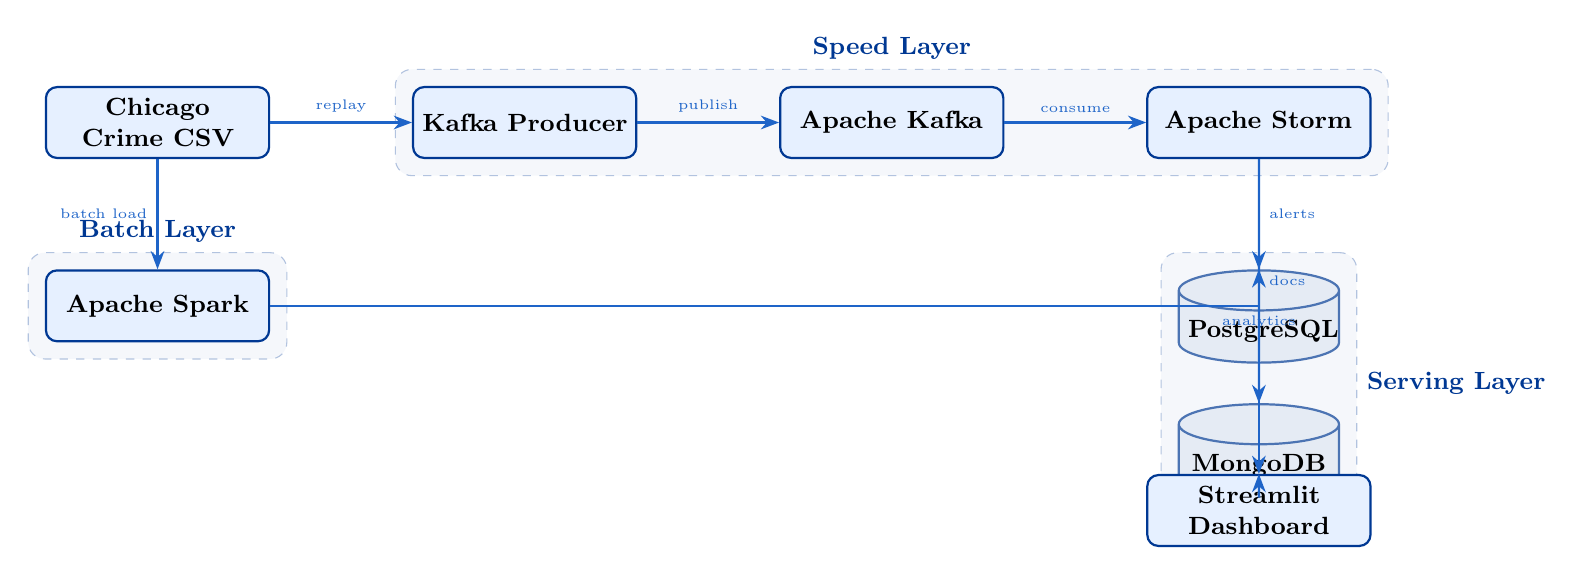
\begin{tikzpicture}[
  node distance=1.0cm and 1.2cm,
  box/.style={rectangle, rounded corners=4pt, draw=nuBlue, thick,
              fill=lightBlue, text width=2.6cm, align=center,
              font=\small\bfseries, minimum height=0.9cm},
  db/.style={cylinder, shape border rotate=90, draw=nuBlue!70, thick,
             fill=nuBlue!10, text width=1.8cm, align=center,
             font=\small\bfseries, minimum height=0.9cm, aspect=0.25},
  arr/.style={-Stealth, thick, color=arrowBlue},
  grp/.style={draw=nuBlue!30, dashed, rounded corners=6pt,
              fill=nuBlue!4, inner sep=6pt},
]

%% Nodes
\node[box] (csv)    {Chicago Crime CSV};
\node[box, right=1.8cm of csv] (prod)   {Kafka Producer};
\node[box, right=1.8cm of prod] (kafka)  {Apache Kafka};
\node[box, right=1.8cm of kafka] (storm) {Apache Storm};

\node[box, below=1.4cm of csv]  (spark)  {Apache Spark};

\node[db, below=1.4cm of storm] (pg)     {PostgreSQL};
\node[db, below=0.5cm of pg]    (mg)     {MongoDB};

\node[box, below=1.4cm of pg]   (ui)     {Streamlit Dashboard};

%% Edges
\draw[arr] (csv)   -- node[above,font=\tiny]{replay} (prod);
\draw[arr] (prod)  -- node[above,font=\tiny]{publish} (kafka);
\draw[arr] (kafka) -- node[above,font=\tiny]{consume} (storm);
\draw[arr] (csv)   -- node[left, font=\tiny]{batch load} (spark);
\draw[arr] (storm) -- node[right,font=\tiny]{alerts} (pg);
\draw[arr] (storm) -- node[right,font=\tiny]{docs} (mg);
\draw[arr] (spark) -| node[below,font=\tiny]{analytics} (pg);
\draw[arr] (pg)    -- (ui);
\draw[arr] (mg)    -- (ui);

%% Layer boxes
\begin{scope}[on background layer]
  \node[grp, fit=(prod)(kafka)(storm), label=above:{\small\color{nuBlue}\textbf{Speed Layer}}] {};
  \node[grp, fit=(spark), label=above:{\small\color{nuBlue}\textbf{Batch Layer}}] {};
  \node[grp, fit=(pg)(mg), label=right:{\small\color{nuBlue}\textbf{Serving Layer}}] {};
\end{scope}
\end{tikzpicture}
\caption{Lambda Architecture — end-to-end data flow}
\end{figure}

\subsection{Technology Stack}

\begin{table}[H]
\centering
\caption{Technology Versions}
\begin{tabular}{lll}
\toprule
\textbf{Component} & \textbf{Technology} & \textbf{Version}\\
\midrule
Batch Processing & Apache Spark (PySpark) & 3.5.0 \\
Stream Broker & Apache Kafka (Confluent) & 7.6.1 (cp-kafka) \\
Stream Processing & Apache Storm & 2.6.2 \\
Coordination & Apache ZooKeeper & bundled \\
Structured Store & PostgreSQL & 16 \\
Document Store & MongoDB & 7.0 \\
Dashboard & Streamlit & 1.41 \\
Producer & Python & 3.12 \\
Orchestration & Docker Compose & — \\
\bottomrule
\end{tabular}
\end{table}

% ═══════════════════════════════════════════════════════════════
\section{Batch Layer — Apache Spark}
% ═══════════════════════════════════════════════════════════════

\subsection{Architecture and Responsibilities}

The batch layer reads all five datasets from disk, enforces explicit schemas, performs preprocessing, computes analytics, and writes results to PostgreSQL. All DataFrames use explicit \texttt{StructType} definitions — schema inference (\texttt{inferSchema=True}) was prohibited.

\subsection{Batch Job Execution}

The batch job is submitted via \texttt{spark-submit} inside the \texttt{spark-master} container:

\begin{lstlisting}[language=bash, caption={Spark Batch Job Submission Command}]
docker compose -f docker/docker-compose.yml exec spark-master \
  /opt/spark/bin/spark-submit \
  --master spark://spark-master:7077 \
  --conf spark.jars.ivy=/tmp/.ivy2 \
  --packages org.postgresql:postgresql:42.7.4 \
  /app/spark/batch_job.py \
  --config /app/config/config.yaml
\end{lstlisting}

\begin{figure}[H]
  \centering
  
\includegraphics[width=0.92\textwidth]{DockerSparkBatchAnalyticsTerminalLogs.png}
  \caption{Spark batch job terminal logs — executor registration, BlockManager init, and completion}
\end{figure}

\begin{figure}[H]
  \centering
  \begin{subfigure}[b]{0.48\textwidth}
    
\includegraphics[width=\textwidth]{SparkUIFullPage.png}
    \caption{Spark Master UI — 1 completed application}
  \end{subfigure}\hfill
  \begin{subfigure}[b]{0.48\textwidth}
    
\includegraphics[width=\textwidth]{SparkApplicationUIFullPage.png}
    \caption{CrimeAnalyticsBatch app detail — FINISHED, 8.3 min}
  \end{subfigure}
  \caption{Apache Spark UI evidence}
\end{figure}

\noindent The Spark UI confirms the \textbf{CrimeAnalyticsBatch} application completed successfully in \textbf{8.3 minutes}, using 2 cores and 1024 MiB executor memory on a single worker node.

\subsection{Analytics Computed}

\subsubsection{Crime Trend Analysis}
Aggregated crime counts grouped by \textbf{year}, \textbf{month}, \textbf{day of week}, and \textbf{hour of day}, written to the \texttt{crime\_trends} table in PostgreSQL.

\begin{figure}[H]
  \centering
  \begin{subfigure}[b]{0.32\textwidth}
    
\includegraphics[width=\textwidth]{Crime Trends by year.png}
    \caption{Crime trends by year (2001–2026)}
  \end{subfigure}\hfill
  \begin{subfigure}[b]{0.32\textwidth}
    
\includegraphics[width=\textwidth]{Crime Trends by months.png}
    \caption{Crime trends by month}
  \end{subfigure}\hfill
  \begin{subfigure}[b]{0.32\textwidth}
    
\includegraphics[width=\textwidth]{Crime Trends by hour.png}
    \caption{Crime trends by hour of day}
  \end{subfigure}
  \caption{Batch layer crime trend analytics from Streamlit dashboard}
\end{figure}

\noindent \textbf{Key observations:}
\begin{itemize}[leftmargin=1.6em]
  \item \textbf{Yearly trend}: Crime counts peaked near 480K–490K in 2001–2002 and show a consistent long-term decline to approximately 200K by 2019–2020, with a slight uptick post-2021, and a sharp drop in 2026 (partial year).
  \item \textbf{Monthly distribution}: Crime is broadly distributed across months (600K–800K range), with mild peaks in the summer months (July–August) consistent with warm-weather crime patterns.
  \item \textbf{Hourly distribution}: Crime is lowest in the early morning hours (4–6 AM, around 110K–150K), rises sharply in the afternoon, and stays elevated through the late evening (midnight peak near 490K–500K).
\end{itemize}

\subsubsection{Arrest Rate Analysis}

The arrest rate (arrests/crimes) is calculated by joining the Crime and Arrests datasets on \texttt{CASE\_NUMBER}, broken down by primary crime type, police district, and race.

\begin{figure}[H]
  \centering
  
\includegraphics[width=\textwidth]{TopArrestRates.png}
  \caption{Top arrest rates by crime type and district — batch analytics output}
\end{figure}

\noindent \textbf{Key findings:}
\begin{itemize}[leftmargin=1.6em]
  \item \textbf{Concealed Carry License Violation} has the highest arrest rate at 0.753 (75.3\%).
  \item \textbf{Interference with Public Officer} (0.3675) and \textbf{Weapons Violation} (0.3286) follow.
  \item Serious crimes like \textbf{Homicide} (0.1317) and \textbf{Public Indecency} (0.1688) have relatively lower arrest rates despite their severity.
  \item \textbf{Other Narcotic Violation} has the highest arrest rate among narcotics-type crimes (0.1879).
  \item Racial categories show arrest rates near 1.0 due to direct join semantics (arrests by definition resulted in arrest).
\end{itemize}

\subsubsection{Geospatial Hotspot Detection (K-Means)}

K-Means clustering ($k=10$) was applied to crime event coordinates (\texttt{LATITUDE}, \texttt{LONGITUDE}) using PySpark MLlib. Cluster centroids and labels are stored in the \texttt{hotspots} PostgreSQL table.

\begin{figure}[H]
  \centering
  \includegraphics[width=0.80\textwidth]{HotspotCentroids.png}
  \caption{K-Means crime hotspot centroids — all clusters concentrated in the Chicago metropolitan area (Illinois, USA)}
\end{figure}

The map shows all 10 cluster centroids aggregated into the Chicago area, confirming spatially coherent clustering. The large red circle represents the density-weighted centroid of the highest-crime cluster covering the downtown and south-side districts.

\subsubsection{Additional Batch Analytics}

\begin{itemize}[leftmargin=1.6em]
  \item \textbf{Violence \& Gunshot Analysis}: Total homicides vs.\ non-fatal shootings by month and district; proportion of incidents involving confirmed gunshot injuries (\texttt{GUNSHOT\_INJURY\_I = `Y'}); top community areas by violence incidence — written to \texttt{violence\_stats}.
  \item \textbf{Sex Offender Proximity Analysis}: Offender density per district using the Police Stations join; records with \texttt{VICTIM\_MINOR = `Y'} flagged for priority reporting — written to \texttt{offender\_density}.
  \item \textbf{Cross-Dataset Correlations}: (1) Violence rate vs.\ total arrest rate grouped by district; (2) Sex offender density vs.\ crime rate grouped by community area — results in \texttt{correlations} table.
\end{itemize}

% ═══════════════════════════════════════════════════════════════
\section{Speed Layer — Kafka \& Apache Storm}
% ═══════════════════════════════════════════════════════════════

\subsection{Kafka Producer}

The Python producer (\texttt{kafka/producer.py}) reads the Crime CSV row-by-row and publishes each record as a JSON message to the \textbf{\texttt{crime\_events}} Kafka topic. The publication rate is configurable via \texttt{config/config.yaml} (default: 1 row/second). Rows missing \texttt{latitude} or \texttt{longitude} are skipped. Each message includes: \texttt{CASE\_NUMBER}, \texttt{DATE}, \texttt{BLOCK}, \texttt{PRIMARY\_TYPE}, \texttt{DISTRICT}, \texttt{ARREST}, \texttt{LATITUDE}, \texttt{LONGITUDE}.

\begin{lstlisting}[language=bash, caption={Starting the Kafka Producer}]
python kafka/producer.py --config config/config.yaml
\end{lstlisting}

\subsection{Storm Topology Design}

The Storm topology implements a 6-bolt pipeline:

\begin{figure}[H]
\centering
\resizebox{\textwidth}{!}{%
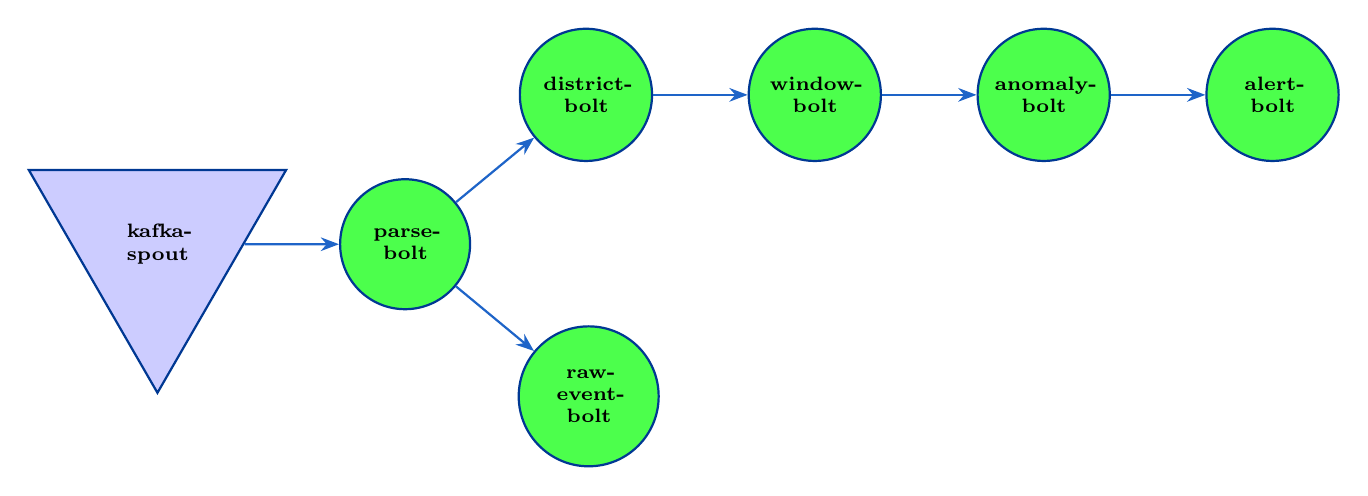
\begin{tikzpicture}[
  node distance=0.6cm and 0.4cm,
  transform shape,
  bolt/.style={
    circle,
    draw=nuBlue,
    thick,
    fill=green!70,
    text width=1.3cm,
    align=center,
    font=\scriptsize\bfseries
  },
  spout/.style={
    regular polygon,
    regular polygon sides=3,
    draw=nuBlue,
    thick,
    fill=blue!20,
    text width=1.1cm,
    align=center,
    font=\scriptsize\bfseries,
    shape border rotate=180
  },
  arr/.style={-Stealth, thick, color=arrowBlue},
]

\node[spout] (kafka) {kafka-spout};

\node[bolt, right=1.2cm of kafka] (parse) {parse-bolt};

\node[bolt, above right=0.7cm and 1.1cm of parse]
(district) {district-bolt};

\node[bolt, below right=0.7cm and 1.1cm of parse]
(rawevent) {raw-event-bolt};

\node[bolt, right=1.2cm of district] (window) {window-bolt};

\node[bolt, right=1.2cm of window] (anomaly) {anomaly-bolt};

\node[bolt, right=1.2cm of anomaly] (alert) {alert-bolt};

\draw[arr] (kafka) -- (parse);
\draw[arr] (parse) -- (district);
\draw[arr] (parse) -- (rawevent);
\draw[arr] (district) -- (window);
\draw[arr] (window) -- (anomaly);
\draw[arr] (anomaly) -- (alert);

\end{tikzpicture}%
}
\caption{Storm topology data flow: kafka-spout $\rightarrow$ parse-bolt $\rightarrow$ district-bolt / raw-event-bolt $\rightarrow$ window-bolt $\rightarrow$ anomaly-bolt $\rightarrow$ alert-bolt}
\end{figure}

\subsubsection{Component Descriptions}

\begin{table}[H]
\centering
\caption{Storm Topology Components}
\begin{tabularx}{\textwidth}{llX}
\toprule
\textbf{Component} & \textbf{Type} & \textbf{Responsibility}\\
\midrule
kafka-spout & Spout & Reads from \texttt{crime\_events} Kafka topic; disables auto-commit \\
parse-bolt & Bolt & Deserialises JSON, validates required fields; discards malformed messages \\
district-bolt & Bolt & Groups events by police district; emits district-tagged tuples \\
raw-event-bolt & Bolt & Stores raw event documents to MongoDB \texttt{crime\_events} collection \\
window-bolt & Bolt & Sliding count window (configurable size/slide); emits per-district counts \\
anomaly-bolt & Bolt & Compares window counts vs.\ threshold; emits alert tuples on breach \\
alert-bolt & Bolt & Persists alert records to PostgreSQL \texttt{alerts} table and MongoDB \texttt{alert\_logs} \\
\bottomrule
\end{tabularx}
\end{table}

\subsection{Storm Topology Submission}

\begin{lstlisting}[language=bash, caption={Building and Submitting the Storm Topology}]
# Build (inside storm-nimbus container)
mvn clean package -DskipTests
# Returns: BUILD SUCCESS in ~2:37 min

# Submit
docker compose -f docker/docker-compose.yml exec storm-nimbus \
  storm jar /storm-app/target/crime-storm-topology-1.0.0.jar \
  edu.nu.crimeanalytics.topology.CrimeAnalyticsTopology \
  crime-analytics-v9
\end{lstlisting}

\begin{figure}[H]
  \centering
  \begin{subfigure}[b]{0.48\textwidth}
    
\includegraphics[width=\textwidth]{BuildAndSubmitStormCommandTerminalLogs.png}
    \caption{Storm topology upload and distributed submission logs}
  \end{subfigure}\hfill
  \begin{subfigure}[b]{0.48\textwidth}
    
\includegraphics[width=\textwidth]{BuildAndSubmitStormCommand2TerminalLogs.png}
    \caption{Maven build success — BUILD SUCCESS in 2:37 min}
  \end{subfigure}
  \caption{Storm build and submission terminal evidence}
\end{figure}

\noindent Image 1 confirms the Storm submitter: (1) set Kafka consumer auto-commit to \texttt{false}, (2) generated a ZooKeeper secret payload, (3) located the Nimbus leader, (4) uploaded the topology JAR, and (5) successfully submitted topology \textbf{crime-analytics-v7} in distributed mode.

\subsection{Storm UI Evidence}

\begin{figure}[H]
  \centering
  
\includegraphics[width=\textwidth]{StormUIFullPage.png}
  \caption{Storm UI — Cluster Summary, Nimbus, Supervisor, and active topology \texttt{crime-analytics-v7}}
\end{figure}

\begin{figure}[H]
  \centering
  \begin{subfigure}[b]{0.55\textwidth}
    
\includegraphics[width=\textwidth]{StormUICrimeAnalyticsFullPage.png}
    \caption{Topology detail — stats, spouts, bolts, and configuration}
  \end{subfigure}\hfill
  \begin{subfigure}[b]{0.42\textwidth}
    
\includegraphics[width=\textwidth]{StormUICrimeAnalyticsTopologyVisualization.png}
    \caption{Storm topology visualization graph}
  \end{subfigure}
  \caption{Storm UI — crime-analytics topology details and DAG visualization}
\end{figure}

\noindent The Storm UI confirms the topology is \textbf{ACTIVE} with:
\begin{itemize}[leftmargin=1.6em,noitemsep]
  \item \textbf{1 worker}, \textbf{11 executors}, \textbf{11 tasks}
  \item \textbf{1,408 MB} assigned memory on a single supervisor
  \item Storm version \textbf{2.6.2}, topology uptime $\sim$50 minutes
  \item \textbf{0 failed} tuples across all windows in the topology stats
  \item All bolts shown as healthy green nodes in the visualization DAG
\end{itemize}

The topology stats table shows 776,700 tuples emitted/transferred across the 3-hour and all-time windows with complete latency of 305,411 ms and 1,060 acked messages.

% ═══════════════════════════════════════════════════════════════
\section{Serving Layer — PostgreSQL \& MongoDB}
% ═══════════════════════════════════════════════════════════════

\subsection{PostgreSQL — Structured Analytics Store}

PostgreSQL stores all structured analytics outputs from both the batch and speed layers:

\begin{table}[H]
\centering
\caption{PostgreSQL Table Schema}
\begin{tabular}{ll}
\toprule
\textbf{Table} & \textbf{Contents}\\
\midrule
\texttt{crime\_trends} & Aggregated counts by year / month / day / hour \\
\texttt{arrest\_rates} & Arrest rate by crime type, district, race \\
\texttt{hotspots} & K-Means cluster centroids and labels \\
\texttt{violence\_stats} & Homicide/shooting metrics by month and district \\
\texttt{offender\_density} & Sex offender count aggregated per district \\
\texttt{correlations} & Cross-dataset correlation results \\
\texttt{alerts} & Real-time anomaly alerts from Storm \\
\bottomrule
\end{tabular}
\end{table}

\begin{figure}[H]
  \centering
  
\includegraphics[width=\textwidth]{LatestAnalytics.png}
  \caption{PostgreSQL alerts table — latest district-level alerts with event count, threshold, and severity}
\end{figure}

\noindent The latest alerts table shows multiple districts generating alerts simultaneously at timestamp \texttt{2026-05-10 14:45:25+00:00}. District 003 leads with 28 events and District 012 with 26 events — both classified as \textbf{HIGH} severity (threshold = 5).

\subsection{MongoDB — Document Alert Store}

MongoDB stores semi-structured alert documents in the \texttt{alert\_logs} collection, providing a flexible audit trail with full JSON payloads.

\begin{figure}[H]
  \centering
  
\includegraphics[width=\textwidth]{MongoDB alert documents.png}
  \caption{MongoDB \texttt{alert\_logs} collection — district alert documents with severity classification}
\end{figure}

\noindent The MongoDB collection confirms Storm's \textbf{AlertBolt} is successfully persisting documents with all required fields: \texttt{district}, \texttt{alert\_timestamp}, \texttt{event\_count}, \texttt{threshold} (5), and \texttt{severity} (HIGH/MEDIUM). District 018 shows 26 events and District 003 shows 19 events — consistent with the PostgreSQL alerts.

% ═══════════════════════════════════════════════════════════════
\section{Infrastructure \& Containerisation}
% ═══════════════════════════════════════════════════════════════

\subsection{Docker Compose Services}

All components are containerised and launched with a single \texttt{docker-compose up} command. The full service inventory is:

\begin{table}[H]
\centering
\caption{Docker Compose Services}
\begin{tabular}{llll}
\toprule
\textbf{Service} & \textbf{Image} & \textbf{Port} & \textbf{Role}\\
\midrule
\texttt{zookeeper} & confluentinc/cp-zookeeper & 2181 & Kafka + Storm coordination \\
\texttt{kafka} & confluentinc/cp-kafka & 29092 & Event broker \\
\texttt{spark-master} & crimeanalytics-spark & 7077, 8080 & Spark cluster master \\
\texttt{spark-worker} & crimeanalytics-spark & — & Spark executor \\
\texttt{storm-nimbus} & storm:2.6.2 & 6627 & Storm cluster master \\
\texttt{storm-supervisor} & storm:2.6.2 & — & Storm worker node \\
\texttt{storm-ui} & storm:2.6.2 & 8081 & Storm web UI \\
\texttt{mongo} & mongo:7.0 & 27017 & Document store \\
\texttt{postgres} & postgres:16 & 5432 & Relational store \\
\texttt{dashboard} & python:3.12-slim & 8501 & Streamlit frontend \\
\bottomrule
\end{tabular}
\end{table}

\begin{figure}[H]
  \centering
  
\includegraphics[width=\textwidth]{DockerRunningContainers.png}
  \caption{Docker Desktop — all 10 containers running simultaneously with MongoDB checkpoint logs}
\end{figure}

\noindent The Docker Desktop screenshot confirms all services are active (green status). MongoDB WiredTiger checkpoint logs show regular snapshots every 60 seconds, confirming the database is healthy and persisting data.

\subsection{Key Configuration Parameters}

All configurable parameters are externalised in \texttt{config/config.yaml}:

\begin{lstlisting}[language=yaml, caption={Key Configuration (config/config.yaml)}]
kafka:
  bootstrap_servers: "kafka:29092"
  topic: "crime_events"
  rate_per_second: 1

storm:
  window_size_seconds: 300      # 5-minute sliding window
  slide_interval_seconds: 10    # slide every 10 seconds
  anomaly_threshold: 5          # alert if >5 events/window

databases:
  postgres_url: "jdbc:postgresql://postgres:5432/crimedb"
  mongo_uri: "mongodb://mongo:27017/crime_analytics"

spark:
  master: "spark://spark-master:7077"
  sample_mode: false
  crime_sample_limit: 500000
\end{lstlisting}

% ═══════════════════════════════════════════════════════════════
\section{Streamlit Dashboard}
% ═══════════════════════════════════════════════════════════════

The Streamlit dashboard (port 8501) unifies both batch and speed-layer outputs into a single live interface. It auto-refreshes and reads from both PostgreSQL and MongoDB.

\begin{figure}[H]
  \centering
  
\includegraphics[width=0.80\textwidth]{StreamlitDashboardFullPage.png}
  \caption{Real-Time Crime Analytics Streamlit dashboard — complete view with Latest Alerts, Top Arrest Rates, Crime Trends (hourly), Hotspot Centroids map, and MongoDB alert documents}
\end{figure}

\noindent The dashboard contains the following panels:

\begin{itemize}[leftmargin=1.6em]
  \item \textbf{Latest Alerts}: Live table of the most recent Storm-generated district alerts with severity classification (HIGH/MEDIUM).
  \item \textbf{Top Arrest Rates}: Ranked table of crime types and districts by arrest rate, sourced from batch analytics.
  \item \textbf{Crime Trends}: Interactive bar charts switchable between Year / Month / Hour views.
  \item \textbf{Hotspot Centroids}: Mapbox-powered map showing K-Means cluster centroids over Chicago.
  \item \textbf{MongoDB Alert Documents}: Live expandable panel showing raw MongoDB alert documents.
\end{itemize}

% ═══════════════════════════════════════════════════════════════
\section{Results Summary}
% ═══════════════════════════════════════════════════════════════

\begin{table}[H]
\centering
\caption{Complete Results Summary}
\begin{tabularx}{\textwidth}{llX}
\toprule
\textbf{Component} & \textbf{Status} & \textbf{Key Output}\\
\midrule
Kafka Producer & \textcolor{green!60!black}{\textbf{WORKING}} & Streaming crime events at 1 row/sec \\
Storm Topology & \textcolor{green!60!black}{\textbf{ACTIVE}} & 11 executors, 0 failures, 776K+ tuples transferred \\
Spark Batch Job & \textcolor{green!60!black}{\textbf{FINISHED}} & Completed in 8.3 min, all 7 tables populated \\
Crime Trends & \textcolor{green!60!black}{\textbf{COMPLETE}} & Year/Month/Hour aggregations in PostgreSQL \\
Arrest Rates & \textcolor{green!60!black}{\textbf{COMPLETE}} & Top: Concealed Carry (75.3\%), Weapons (32.9\%) \\
K-Means Hotspots & \textcolor{green!60!black}{\textbf{COMPLETE}} & 10 clusters, all in Chicago metro area \\
PostgreSQL Alerts & \textcolor{green!60!black}{\textbf{LIVE}} & 20+ districts generating HIGH/MEDIUM alerts \\
MongoDB Documents & \textcolor{green!60!black}{\textbf{LIVE}} & Alert documents with full JSON payloads \\
Streamlit Dashboard & \textcolor{green!60!black}{\textbf{RUNNING}} & 5 panels, live refresh from both databases \\
Docker Compose & \textcolor{green!60!black}{\textbf{COMPLETE}} & 10 services, single-command launch \\
\bottomrule
\end{tabularx}
\end{table}

% ═══════════════════════════════════════════════════════════════
\section{Challenges and Solutions}
% ═══════════════════════════════════════════════════════════════

\subsection{Spark \texttt{--packages} / Ivy Cache in Container}

\textbf{Symptom}: \texttt{spark-submit} with \texttt{org.postgresql:postgresql} failed when Ivy tried to write under a missing or non-writable cache path inside the Docker container.

\textbf{Fix}: Use a writable Ivy root: \texttt{--conf spark.jars.ivy=/tmp/.ivy2}, reflected in the submission command. This allows the Maven dependency resolver to download the JDBC driver at runtime.

\subsection{Ghost Alerts — Threshold vs.\ Simulation Rate}

\textbf{Symptom}: Dashboard alert tables stayed empty despite an active Kafka producer.

\textbf{Cause}: The default threshold was too high for the replay pattern, as many districts split the traffic resulting in low per-district counts per window.

\textbf{Fix}: Tuned Storm environment variables: \texttt{WINDOW\_SIZE\_SECONDS=300}, \texttt{SLIDE\_INTERVAL\_SECONDS=10}, \texttt{ANOMALY\_THRESHOLD=5}. This produced the rich alert output visible in both PostgreSQL and MongoDB.

\subsection{Kafka Consumer Lock on Topology Resubmission}

\textbf{Symptom}: A newly submitted topology consumed nothing from Kafka despite the producer running.

\textbf{Cause}: The older topology instance remained attached to the same Kafka consumer group. With a single partition, only one consumer receives messages.

\textbf{Fix}: Kill superseded topologies (\texttt{storm kill <name>}) before relying on a new submission. This explains the versioned naming (v7, v9) visible in the Storm UI topology IDs.

\subsection{Large Local CSV Files}

\textbf{Challenge}: The crimes extract is a multi-million-row file; repeated full scans during development iterations are slow on a laptop and stress Docker disk I/O.

\textbf{Mitigation}: Spark column pruning and write-once batch job keep recomputation explicit. Optional limits in \texttt{config.yaml} (\texttt{crime\_sample\_limit}, \texttt{sample\_mode}) support faster development cycles.

\subsection{Dirty Schema Names and Weak Join Keys}

\textbf{Challenge}: Chicago exports use human-readable headers (spaces, mixed case) and joins such as crime↔arrest depend on case-number alignment. Violence and sex-offender extracts use different key conventions.

\textbf{Mitigation}: Centralised rename+cast steps, \texttt{dropDuplicates} on arrests, and documented limitations (e.g., offender-to-district hashing) instead of silent wrong joins.

\subsection{Container Orchestration on Windows/WSL2}

\textbf{Challenge}: Coordinating ZooKeeper, Kafka, Storm, Spark, two databases, and Streamlit with correct ports, dependencies, and environment variables is error-prone on Windows/WSL2.

\textbf{Mitigation}: A single \texttt{docker/docker-compose.yml} encodes service order, Storm environment variables, and published ports. All 10 services launched successfully as shown in the Docker Desktop screenshot.

% ═══════════════════════════════════════════════════════════════
\section{Limitations and Future Improvements}
% ═══════════════════════════════════════════════════════════════

\begin{itemize}[leftmargin=1.6em]
  \item \textbf{Operational metrics}: Surface Kafka consumer lag, Storm bolt execute latency, and end-to-end alert delay as quantitative streaming-performance metrics.
  \item \textbf{Scale-out}: Increase Kafka topic partitions and Storm worker count for higher-throughput stress testing.
  \item \textbf{Richer anomaly detection}: Implement per-district, per-time-of-week baselines instead of a single global threshold; add optional seasonal adjustment.
  \item \textbf{Geospatial refinement}: H3-grid-based hotspots and reproducible CRS handling for more accurate centroid maps.
  \item \textbf{Schema evolution}: Implement schema registry (Confluent Schema Registry) for Kafka message versioning as datasets update.
  \item \textbf{Cloud deployment}: Package as a Kubernetes Helm chart for production deployment on AWS/GCP.
\end{itemize}

% ═══════════════════════════════════════════════════════════════
\section{AI Use Disclosure}
% ═══════════════════════════════════════════════════════════════

As per the course's academic integrity policy, we disclose that \textbf{generative AI assistance} (Claude, GitHub Copilot) was used to scaffold, debug, and document parts of this project — including README structure, Docker/Spark troubleshooting notes, LaTeX report formatting, and code review-style refactors. All architectural decisions, implementation logic, and analytical interpretations were made by the project team.

% ═══════════════════════════════════════════════════════════════
\section{Conclusion}
% ═══════════════════════════════════════════════════════════════

This project successfully implements a full Lambda Architecture for real-time crime analytics on Chicago's public safety data. The system demonstrates:

\begin{itemize}[leftmargin=1.6em]
  \item \textbf{Batch intelligence}: PySpark processed millions of crime records in 8.3 minutes, producing seven analytics tables covering trends, arrest rates, violence statistics, offender density, geospatial hotspots, cross-dataset correlations, and real-time alerts.
  \item \textbf{Real-time awareness}: The Kafka+Storm pipeline successfully detects district-level crime anomalies within sliding 5-minute windows, generating HIGH and MEDIUM severity alerts persisted to both PostgreSQL and MongoDB.
  \item \textbf{Production-grade engineering}: Docker Compose orchestrates 10 services from a single command; all parameters are externalised; error handling is embedded throughout the topology.
  \item \textbf{Unified visibility}: The Streamlit dashboard merges both layers into one coherent interface accessible to non-technical stakeholders.
\end{itemize}

The system mirrors the architecture of production law-enforcement analytics platforms and demonstrates that open-source big-data technologies (Spark, Kafka, Storm) can deliver meaningful public-safety intelligence at city scale.

% ═══════════════════════════════════════════════════════════════
\section*{Project Structure}
\addcontentsline{toc}{section}{Project Structure}
% ═══════════════════════════════════════════════════════════════

\begin{lstlisting}[language=bash, caption={Repository Folder Structure}]
CrimeAnalytics/
├── config/         # config.yaml (Kafka, DBs, windows, thresholds)
├── dashboard/      # streamlit_app.py
├── db/             # postgres_init.sql, mongo_setup.py
├── docker/         # docker-compose.yml, Dockerfiles
├── kafka/          # producer.py (CSV replay)
├── spark/          # batch_job.py (PySpark analytics)
├── storm/          # Java topology: spouts/, bolts/, topology/
├── Figs/           # Report screenshots and terminal evidence
├── requirements.txt
└── README.md
\end{lstlisting}

\begin{infobox}[Reproducible Demo Runbook]
\begin{enumerate}[leftmargin=1.4em, noitemsep]
  \item \texttt{docker compose -f docker/docker-compose.yml up -d} \hfill\textit{Start all services}
  \item Submit Spark batch job (see §5.2) \hfill\textit{Populates PostgreSQL}
  \item \texttt{mvn clean package} then submit Storm JAR (see §6.2) \hfill\textit{Activates streaming}
  \item \texttt{python kafka/producer.py --config config/config.yaml} \hfill\textit{Starts event replay}
  \item Open \url{http://localhost:8501} (dashboard), \url{http://localhost:8081} (Storm UI)
\end{enumerate}
\end{infobox}

\vfill
\noindent\rule{\textwidth}{0.5pt}\\
{\small \textbf{Submitted by:} Muhammad Mobin (21I-0794) \& Muhammad Nouman Hafeez (21I-0416) $\cdot$ CS-A $\cdot$ FAST-NUCES Islamabad $\cdot$ CS4109 Big Data Analytics $\cdot$ May 2026}

\end{document}